\chapter{Characterizing the Two-Qubit Processor} \label{chapter:processor_characterization}

After having detailed the design of the processor and the measurement techniques employed in this work, we discuss in this chapter how we characterize the processor and demonstrate the basic functionality that we need to run meaningful quantum algorithms. In particular we show how we implement and characterize the universal $\sqrt{i\mathrm{SWAP}}$ two-qubit quantum gate with 90\% fidelity, similar to the gate used in the following chapter to run the Grover search algorithm.

\smallskip

The chapter begins with the choice of the different working points during operation, based on the measurement of the basic qubit coherence properties and readout fidelities as a function of the qubit frequency.   Then, single-qubit microwave gates are characterized. Afterwards, we discuss the generation and characterization of entanglement by quantum state tomography, and perform a test of the so-called CHSH Bell inequality. Finally, we discuss in detail how we characterize our $\sqrt{i\mathrm{SWAP}}$ gate by quantum process tomography: we explain how we estimate and/or fit the microwave pulse errors in order to remove the tomographic errors and obtain a fidelity that characterizes the gate alone.

\section{Individual Qubit and Readout Characterization \\ Choice of the Working Points}

The first step in the characterization of the processor consists in obtaining all relevant qubit and readout parameters, as described in chapter \ref{chapter:measurement}. For this, we perform a set of measurements from which we obtain the qubit frequencies, anharmonicities, junction asymmetries, inter-qubit coupling, coupling to the microwave drive lines, coupling of each qubit to its readout, as well as qubit relaxation and dephasing times. Most of these parameters are measured for a range of qubit frequencies in order to pick up the best working points for implementing the gate. 

\subsubsection{Qubit Frequency, Anharmonicity and Asymmetry}

To obtain the Josephson and charging energies as well as the junction asymmetries of the qubits, we perform spectroscopic measurements of the single-photon $\ket{0}\to \ket{1}$ and two-photon $\ket{0}\to\ket{2}$ qubit transitions at different values of the external magnetic flux $\Phi_{ext}$, as described in section \ref{section:qubit_spectroscopy}. By fitting equations (\ref{eq:cpb_energies}) and (\ref{eq:josephson_energy_modulation}) to the resulting values $\omega_{01}(\Phi_{ext})$ and $\omega_{02}(\Phi_{ext})$ (see fig. \ref{fig:qubit_parameters}a) we obtain all relevant qubit parameters. For our processor, these are $E_J^I / h = 36.2\; \mathrm{GHz}$, $E_c^I / h = 0.98 \; \mathrm{GHz}$ and $E_J^{II} / h = 43.1\; \mathrm{GHz}$, $E_C^{II} / h = 0.87 \; \mathrm{GHz}$ for the Josephson and charging energies of the two qubits, yielding anharmonicities $\alpha^I\approx 245\;\mathrm{MHz}$ and $\alpha^{II}\approx 220\;\mathrm{MHz}$. For the qubit junction asymmetries, we obtain $d^I = 0.2$, $d^{II} =  0.35$.

\subsubsection{Readout Parameters}

To obtain the resonance frequencies and quality factors of the readout resonators we perform a simple measurement of the $S_{11}$ reflection coefficient. The resulting frequencies are $f_R^I = 6.84 \; \mathrm{GHz}$ and $f_R^{II} = 6.70 \; \mathrm{GHz}$ with quality factors $Q^I \simeq Q^{II} = 730$. We measure the Kerr nonlinearity $K$ of the resonators, as defined by eq. \ref{eq:KNR}, by following the procedure given in \citep[p. 166]{palacios-laloy_superconducting_2010} and obtain $K^I \simeq K^{II}= -2.3\pm 0.5 \times 10^{-5}$.

\subsubsection{Qubit/Readout Coupling}

The coupling of each qubit to its readout resonators is determined by spectroscopically measuring the avoided level crossing between them. For this, we perform a series of spectroscopic measurements of the resonator while tuning the qubit frequency from below the resonator frequency to above it. Performing such a measurement on a chip identical to the one used in the main experiment reported here yields a coupling coefficients $g_{01}^I \simeq g_{01}^{II} = 2\pi\cdot 50 \; \mathrm{MHz}$.

\subsubsection{Qubit Parameter Survey} \label{section:qubit_parameter_survey}

\begin{figure}[p]
   \centering
	 \rotatebox{-90}{\includegraphics[width=0.8\textheight]{"./data/ct5/qubits - parameter surveys/qubit_parameters_new"}}
	 \caption{Parameter survey of the two qubits. a) Experimental (dots) and fitted (lines) qubit $f_{01}^{I,II}$ and $f_{12}^{I,II}$ frequencies. b) Experimental (red crosses) and expected (lines) relaxation rates $\Gamma_1$ of the qubits. The calculated contributions are those of the Purcell effect $\Gamma_\mathrm{Purcell}$ (magenta), the relaxation due to capacitive coupling to the flux line $\Gamma_{fl,c}$ (green) and their sum (blue). c) Rabi frequency $\Omega_\mathrm{Rabi}^{I,II}$ at a fixed drive amplitude, measured (red crosses) and modeled using eq. (\ref{eq:qubit_drive_voltage}). d) Readout contrast $c_{01}$ of the two qubits, for a range of qubit frequencies. The chosen processor working points $f_{01,r}^{I,II}$, $f_{01,m}^{I,II}$ and $f_{01,c}^{I,II}$ are also indicated with purple disks.}
	 \label{fig:qubit_parameters}
\end{figure}

In order to determine the optimal working points for our processor, we characterize the properties of the qubits in a large frequency window. For this, we perform an automated measurement of the transition frequencies $\omega_{01}$ and $\omega_{02}$, of the readout contrasts $c$,  and of the relaxation rate $\Gamma_1$ of each qubit at different values of the magnetic flux $\Phi_{ext}$. The results are summarized in fig \ref{fig:qubit_parameters}. The expected Purcell relaxation rates $\Gamma_\mathrm{Purcell}^{I,II}$ as given by eq. (\ref{eq:purcell_rate}) are shown in magenta and are much lower than the actual observed rates for the two qubits. We can also take into account qubit relaxation $\Gamma_{fl,c}^{I,II}$ due to a capacitive coupling of the qubit electrodes to the fluxline, which can be calculated using eq. (\ref{eq:charge_relaxation_rate}). In order to reach the lowest measured relaxation rate, we fit a capacitive coupling $C_{g,fl} = 2\;\mathrm{fF}$ to the fluxline that we model as two parallel $50\;\Omega$ transmission lines equivalent to an effective impedance $Z_{fl} = 25\;\Omega$. However, this still cannot explain quantitatively the observed data: hence there must be at least one additional relaxation channel in our design that we have not captured. Since the observed Rabi frequencies of the qubits are in agreement with the expected Purcell filtering of the readout resonator, we can rule out additional relaxation through the readout gate circuit, leaving only microscopic channels or the coupling of the qubit to an unknown external impedance as possible causes of the observed relaxation.

\smallskip

The observed qubit Rabi frequencies $\Omega_\mathrm{Rabi}^{I,II}$ at a fixed drive input voltage $V_{in}$ agree well with eq. (\ref{eq:qubit_drive_voltage}). The best fit to this model, obtained with the measured resonator frequencies and quality factors and with only the input voltage $V_{in}$ as a fitting parameter, is shown in blue and agrees well with the measurement data for both qubits, confirming that the filtering through the readout resonator works.

\smallskip

As expected, the readout contrast increases when decreasing the qubit-resonator detuning $\Delta$, in accordance with an increase of the dispersive frequency shift given by eq. (\ref{eq:stark_shift}).

\smallskip

The qubit dephasing rates $\Gamma_\phi^{I,II}$ (which are not shown in the plot since they have not been measured systematically) vary between $2-4\;\mathrm{MHz}$ and do not show a clear dependence on the qubit frequencies.

\subsubsection{Choice of Manipulation and Readout Working Points}

Having characterized all parameters of the individual qubits as a function of $\omega_{01}^I$ and $\omega_{01}^{II}$, we can choose the frequency working points for qubit manipulation and readout, and place them on fig. \ref{fig:qubit_parameters}. For single-qubit manipulation and parking, we choose \mbox{$\omega_{01,m}^I/2\pi = 5.247\;\mathrm{GHz}$} and \mbox{$\omega_{01,m}^{II}/2\pi = 5.125\;\mathrm{GHz}$}, where we have relaxation times \\ \mbox{$T_1^I(\omega_{01,m}^I) \approx 440\;\mathrm{ns}$} and \mbox{$T_1^{II}(\omega_{01,m}^{II})\approx 520\;\mathrm{ns}$}. For qubit readout, we choose \mbox{$\omega_{01,r}^I \approx 6.2\;\mathrm{GHz}$} and \mbox{$\omega_{01,r}^{II}\approx 6.0\;\mathrm{GHz}$}, where we have single-shot readout contrasts \mbox{$c_{01}^I(\omega_{01,r}^I)\approx 75\%$} and \mbox{$c_{01}^{II}(\omega_{01,r}^{II})\approx 73\%$}.

\section{Two-Qubit Readout Characterization} \label{section:readout_matrix}

\begin{SCfigure}[1.0][ht!]
	\centering
	\includegraphics[width=0.5\textwidth]{"./data/ct5/2011_04_21 - grover and tomo/good_data/readout_matrix_no_shelving"}
	\caption{The measured readout matrix of our two-qubit processor. Shown are the conditional measurement probabilities $p_m(x_{1}x_{2}|\ket{y_{1}y_2})$, with $x_1,x_2,y_1,y_2\in\{0,1\}$. The diagonal elements correspond to the readout fidelities of the four basis states. The single qubit readout fidelities as obtained from the matrix are $p_m^I(0*|\ket{00})=0.88$, $p_m^I(1*|\ket{10})=0.85$, $p_m^{II}(*0|\ket{00})=0.9$ and $p_m^{II}(*1|\ket{01})=0.85$, the readout crosstalks are $p_m(0*|\ket{00}) - p_m(0*|\ket{01})=-0.01$, $p_m(1*|\ket{10}) - p_m(1*|\ket{11})=-0.02$, $p_m(*0|\ket{00}) - p_m(*0|\ket{10})=0$ and $p_m(*1|\ket{01}) - p_m(*1|\ket{11})=-0.01$.}
	\label{fig:readout_matrix_no_shelving}
\end{SCfigure}

The errors of an n-qubit readout are fully characterized by giving a complete set of switching probabilities $p_m(x_{1}x_{2}\hdots x_n|\ket{y_{1}y_{2}\hdots y_n})$, which correspond to the probability of obtaining a readout outcome $x_{1}x_{2}\hdots x_{n}$ after preparing an input state $\ket{y_{1}y_{2}\hdots y_{n}}$, with $x_i,y_i\in \{0,1\}$. 

\smallskip

The single-qubit fidelities $p_m(0|\ket{0})$ and $p_m(1|\ket{1})$ can be simply obtained from an s-curve measurement, as explained in section \ref{section:qubit_readout}. In order to calibrate the two-qubit readout errors, we perform an experiment at the readout working points indicated above, where we measure the full set of conditional probabilities $p(x|\ket{y})$ with $\{x,y\}\in\{00,01,10,11\}$. For this purpose, the qubit register is initialized in each basis state before performing a simultaneous readout of the two qubits. By repeating and averaging the resulting outcomes we obtain the full set of conditional readout probabilities, which we plot as a $4\times 4$ readout matrix $\mathbf{R}$, shown in fig. \ref{fig:readout_matrix_no_shelving}. Here, we assume that the state preparation errors of the input states, e.g. due to thermal excitation of the qubits out of the $\ket{0}$ state, erroneous single-qubit pulses or leakage to the qubit state $\ket{2}$, are sufficiently small so that they can be neglected. From the readout matrix, all conditional and unconditional readout fidelities as well as the readout crosstalk can be calculated. We can correct any measured set of probabilities $\mathbf{p}_R=(p_{00},p_{01},p_{10},p_{11})$ for readout errors by simply multiplying it with the inverse of $\mathbf{R}$, such that $\mathbf{p}_R^{corr}=\mathbf{p}_R\cdot \mathbf{R}^{-1}$. For all experiments discussed in the remainder of this chapter, we will always correct readout errors by this method (unless indicated otherwise) and interpret $\mathbf{p}_R^{corr}$ as the occupation probabilities of the four computational basis states.

\section{Single-Qubit Gate Characterization}

\begin{figure}[ht!]
	\centering
		\includegraphics[width=\textwidth]{"./data/ct5/2010_12_01 - iq tomography/iq_tomography_analysis"}
	\caption{Characterization of single-qubit XY control. a) Measured state $\ket{1}$ occupation probability after preparing a qubit in one of the states $\ket{1}$, $1/\sqrt{2}(\ket{0}+\ket{1})$ or $1/\sqrt{2}(\ket{0}+i\ket{1})$ and subjecting it to a microwave drive pulse of constant duration and variable phase: $a(t) = V_I\cdot\cos{\omega_{rf}t}+V_Q\cdot\sin{\omega_{rf}t}$.  b) Best fit to the data of  the model given by eq. (\ref{eq:iq_model}). c) Difference between measured data and fit (magnified x8)}
	\label{fig:single_qubit_iq_control}
\end{figure}

To perform arbitrary single-qubit operations -- as needed for implementing a quantum algorithm,  for characterizing a two-qubit gate by quantum process tomography, or more simply for preparing a particular state and characterizing it by quantum state tomography-- we need to implement a complete set of rotations like  $X$, $Y$ and $Z$. As already explained, rotations in the $XY$-plane are implemented through microwave drive pulses, where the phase of the drive pulse relative to an arbitrary reference determines the rotation axis and the amplitude the effective Rabi frequency. To characterize these drive pulses, we prepare a single qubit in the states $\ket{1}$, $1/\sqrt{2}(\ket{0}+\ket{1})$ or $1/\sqrt{2}(\ket{0}+i\ket{1})$, and subject it afterward to a single microwave pulse of varying amplitude and phase: this pulse of form $V(t) = V_Ia(t)\cdot\cos{\omega_{rf}t}+V_Qa(t)\cdot\sin{\omega_{rf}t}$, is obtained by I-Q mixing the microwave carrier at $\omega_{rf}$  to DC $V_Ia(t)$ and $V_Qa(t)$ pulse envelopes with the same constant duration, with Gaussian rise and fall, and with increasing amplitudes $V_I$ and $V_Q$. We then measure and plot  (see fig. \ref{fig:single_qubit_iq_control}) the occupation probability of state $\ket{1}$  as a function $V_I$, $V_Q$. The qubit that was prepared in state $\ket{1}$ shows a rotational-invariant switching probability pattern, which is indeed what one expects for a qubit prepared in either $\ket{0}$ or $\ket{1}$. On the other hand, the switching probability distributions of the qubits prepared in the states $1/\sqrt{2}(\ket{0}+\ket{1})$ and $1/\sqrt{2}(\ket{0}+i\ket{1})$ are almost symmetric with respect to the axis along which the qubit has been prepared. Performing a fit of the model
%
\begin{equation}
\ket{\psi_{out}}= \exp{\left(-i\frac{\varphi}{2}[\cos{(\alpha+\alpha_0)}\hat{\sigma}_x+\sin{(\alpha+\alpha_0)}\hat{\sigma}_y]\right)}\ket{\psi_{in}}, \label{eq:iq_model}
\end{equation}
%
with $\alpha=\mathrm{atan}{( c_Q Q/c_I I)}$, to the measured occupation probability,  we obtain the fitting parameters  $c_I$, $c_Q$, $\varphi$ , and the overall gate phase error $\alpha_0 \le 2.8^\circ $. This measurements demonstrate our ability to prepare and drive the qubit along arbitrary axes of the Bloch sphere. Nevertheless, the phase error $\alpha_0$ depends on the rotation angle $\varphi$ due to mixer imperfections,  as can be seen on figure  \ref{fig:single_qubit_iq_control} where the error is larger for $\pi/2$ pulses. Consequently, we have also calibrated separately $\pi$ and $\pi/2$ pulses for the experiments, as reported below.

\smallskip

\begin{SCfigure}[1.0][ht!]
	\centering
	\includegraphics[width=0.7\textwidth]{./data/phase_error_analysis}
	\caption{Measured (dots) and fitted (line) occupation probability of state $\ket{1}$ at the manipulation working point after subjecting the qubit to a $X_{\pi/2}\Phi_{\pi/2}$ pulse sequence, as a function of $\Phi$. Red data corresponds to an uncorrected drive pulse, resulting in a phase error $\epsilon_\Phi\approx 7.66^\circ$, whereas blue data corresponds to a corrected drive pulse, resulting in $\epsilon_\Phi' \approx 0.09^\circ$.}
	\label{fig:ape}
\end{SCfigure}

We calibrate the length of our $\pi/2$ and $\pi$ pulses by performing a Rabi experiment, as explained in section \ref{section:qubit_rabi}. We then correct errors in the direction $\Phi$ of the rotation axis by performing a so-called {\it amplified pulse error} sequence \citep{lucero_reduced_2010}. This sequence consists of a $X_{\pi/2}$ pulse followed by a $\Phi_{\pi/2}$ pulse, where $\Phi$ gives the rotation axis of the second pulse. Performing it for different values of $\Phi$, measuring the state $\ket{1}$ occupation probability afterwards, and fitting the resulting curve to a model of the form $p(\ket{1}) = p_0+p_a\cos{(\Phi-\epsilon_\Phi)}$ allows us then to extract both amplitude errors $\epsilon_a=|p_a-0.5|$ and phase errors $\epsilon_\Phi$. These can be further amplified by interposing a number of identity operators $X_{\pi/2}X_{-\pi/2}$ between the two drive pulses, which we do not do in this work, however. The phase shift $\epsilon_\Phi$ of the minimum of the curve with respect to $\pi$ is due to both the leakage to the Transmon state $\ket{2}$ and the drive-induced frequency shift discussed in section \ref{section:qubit_driving}. The first source of error could be corrected by using special DRAG drive pulses \citep{lucero_reduced_2010}, which we don't do in this work. We correct the second source of errors by detuning the drive frequency as explained in section \ref{section:qubit_driving}. Figure \ref{fig:ape} shows an exemplary APE measurement for qubit I, where the phase error for an uncorrected qubit pulse is $\epsilon_\Phi\approx 7.66^\circ$, which gets reduced to $\epsilon_\Phi'\approx 0.09^\circ$ by detuning the qubit drive frequency by $\Delta f_{dr}=-4\;\mathrm{MHz}$. We are thus able to perform single-qubit pulses with an angular precision $\le 1^\circ$, both in angle and in rotation direction, just after a calibration. Nevertheless, the experiment tends to drift and the errors thus tend to be larger when performing long measurements.

\section{Demonstrating Two-Qubit Entanglement}

We first choose the working point at which the two qubits will be resonantly coupled to perform a $\sqrt{i\mathrm{SWAP}}$ gate.
Because the coupling strength $g_{qq}$ defined by eq. \ref{eq:cqed_qubit_interaction_hamiltonian} depends very weakly on this working point in the vicinity of the manipulation points defined above, we choose for a sake of simplicity to shift the frequency of only one qubit. So we will displace qubit I by $-122\;\mathrm{MHz}=30 g_{qq}/2\pi$ (see below) from its manipulation point at $\omega_{01,m}^I/2\pi = 5.247\;\mathrm{MHz}$ to the manipulation point of qubit II at  $\omega_{01,m}^{II}/2\pi = 5.125\;\mathrm{MHz}$.

\subsection{Coupling Strength Between Qubits} \label{section:Coupling_Strength_Between_Qubits}
\begin{figure}[ht!]
	\centering
	\begin{tabular}{l}
	  a) \\
		\includegraphics[width=0.67\textwidth]{"./material/figures/measurement/anticrossing_spectroscopy"} \\
		b) \\
		\includegraphics[width=0.7\textwidth]{"./data/ct5/2011_04_11 - anticrossing/qubit_anticrossing"}
	\end{tabular}
	\caption{ Measurement of the two-qubit anticrossing at the coupling working point. a) Pulse sequence used. b - left) Switching probability of readout II as a function of flux $\Phi_{ext}^I$ and frequency $f_d$ of the spectroscopic pulse applied to qubit I . b - right) Cut at the middle of the anticrossing (dotted line in the 2D plot)  yielding $2g_{qq}/2\pi=8.3\;\mathrm{MHz}$. }
	\label{fig:qubit_anticrossing}
\end{figure}

We then measure the qubit-qubit coupling strength $g_{qq}$ at the coupling working point. For that purpose, the frequency $\omega_{01}^I$ of qubit I is tuned with the flux $\Phi_{ext}^I$ across the fixed frequency $\omega_{01}^{II}$ of qubit II; at each frequency a spectroscopic pulse is applied to qubit I, and qubit II is read out. Plotting the switching probability of  readout II, one obtains the anticrossing shown on fig. \ref{fig:qubit_anticrossing}: close to resonance, the eigenstates of the two-qubit system approach the two Bell states $\ket{\Psi_\pm} = 1/\sqrt{2}(\ket{10}\pm\ket{01})$, which are both excited by the drive of qubit I and detected by measuring qubit II. Hence we observe two spectroscopic lines corresponding to the two transitions $\ket{00}\to 1/\sqrt{2}(\ket{01}+\ket{10})$ and $\ket{00}\to 1/\sqrt{2}(\ket{01}-\ket{10})$. Their maximum separation yields the coupling strength $2g_{qq}/2\pi = 8.3\;\mathrm{MHz}$.

\subsection{Creation of Entanglement} \label{section:creation_of_entanglement}

\begin{figure}[p]
	\begin{tabular}{l}
	a) \\ \multicolumn{1}{c}{\hspace{0.6cm}\includegraphics[width=0.55\textwidth]{"./material/figures/measurement/qubit_swap"}} \\
	b) \\ \multicolumn{1}{r}{\includegraphics[width=0.7\textwidth]{"./material/papers/iswap/figures/swap_raw_and_corrected"}}
	\end{tabular}
	\caption[]{a) Pulse sequence used to create an entangled two-qubit state using a non-adiabatic pulse that brings the qubits in resonance for a well-defined time. b) State occupation probabilities for the two-qubit register during a coherent energy swap. b1) Shows the raw state probabilities corresponding to the states $\ket{00}$, $\ket{01}$, $\ket{10}$ and $\ket{11}$, b2) shows the same data corrected for the limited visibility of each qubit readout and b3) shows the fully corrected readout probabilities where we account for both visibility and inter-qubit readout crosstalk errors.}
	\label{fig:swap_raw_and_corrected}
	\label{fig:qubit_swap_pulse_sequence}
\end{figure}


Knowing the qubit-qubit coupling strength, we then perform a coherent swapping operation between the qubits by preparing the register either in $\ket{01}$ or $\ket{10}$ by shifting non adiabatically the frequency of qubit I down to that of qubit II during a well defined time, and by measuring the two-qubit register directly afterward. The flux pulses used for this are optimized as explained in section \ref{section:fast_flux_pulses}. The expected evolution operator of the process is
%
\begin{equation}
U(t)=\exp{\left(i\theta_I\hat{\sigma}_z^I+i\theta_{II}\hat{\sigma}_z^{II}\right)}\left(\begin{array}{cccc}
1 & 0 & 0 & 0\\
0 & \cos{(tg_{qq})} & -i\sin{(tg_{qq})} & 0\\
0 & -i\sin{(tg_{qq})} & \cos{(tg_{qq})} & 0\\
0 & 0 & 0 & 1\end{array}\right), \label{eq:swap_evolution_operator_main}
\end{equation}
%
where $\theta_{I,II}$ are dynamical phases accumulated by each qubit due to their frequency shift with respect to their manipulation and parking point  during the operation. For qubit I, this shift is directly applied on purpose and is large, whereas for qubit II, it is due to the flux crosstalk and is small. As can be seen on eq. \ref{eq:swap_evolution_operator_main}, the register state is expected to oscillate between the $\ket{01}$ and $\ket{10}$ states with frequency $g_{qq}$. The states $\ket{00}$ and $\ket{11}$ are not affected by the interaction except for a phase factor.

\smallskip

Figure \ref{fig:qubit_swap_pulse_sequence} shows the experimental sequence used as well as the results obtained as a function of the coupling duration. Shown are the raw readout outcomes (i.e. without any corrections), the readout probabilities corrected for the individual readout visibilities, and  the qubit state probabilities $p(\ket{00})$, $p(\ket{01})$, $p(\ket{10})$ and $p(\ket{11})$ obtained after correcting the outcomes for both readout visibilities and crosstalk using the readout matrix $\mathbf{R}$ of fig. \ref{fig:readout_matrix_no_shelving}. The data shows the expected swap between states $\ket{01}$ and $\ket{10}$, as well as the reduction of the swapping amplitude, caused by relaxation and dephasing. The swapping frequency $2g_{qq}/2\pi = 8.3\;\mathrm{MHz}$ agrees with the value obtained from the spectroscopic measurement. Figure \ref{fig:swap_raw_and_corrected}c also shows a master equation simulation of the experiment using the Hamiltonian and the Lindblad super-operators discussed in section \ref{section:master_equation}. This simulation involves the measured $g_{qq}$ and the measured relaxation rates of the qubits  at the coupling working point, whereas dephasing rates are left as free fitting parameters. The reason for this is that the effective dephasing rate of the two-qubit register in the $\{\ket{01},\ket{10}\}$ sub-space is very different from the dephasing rates of individual qubits. Indeed, the transition frequency between the two eigenstates $\ket{\psi_\pm}=1/\sqrt{2}(\ket{01}\pm\ket{10})$ at resonance, i.e. $\omega_{01}^{\pm}=\omega_{01}^{I,II}\pm\sqrt{4g_{qq}^2+\Delta^2}/2\approx \omega_{01}^{I,II}\pm g_{qq} +\Delta^2/8g_{qq}$, is sensitive to variations of the frequency detuning $\Delta$ to second order only. Hence, the effective dephasing rate of the two-qubit system is much lower than the single-qubit dephasing rates. The computation of the transversal relaxation super-operator in the $\{\ket{01},\ket{10}\}$ sub-space is made complicated by the 1/f nature of the $\Delta$ noise as well as by the non-Gaussian character of the noise in $\Delta^2$.  Consequently, we have chosen to reproduce the observed swapping using purely phenomenological and independent dephasing super-operators in the $\{\ket{0},\ket{1}\}$ Hilbert spaces of each qubit. As can be seen, this purely phenomenological model agrees very well with the experimental data with $\Gamma_{\phi}^{I,II}=2\mu$s, probably because dephasing has only a small effect.


\subsection{Quantum State Tomography}

The experiments that we describe in the following sections will require us to determine experimentally the density matrix of the two-qubit register. The method that we use for this is called {\it quantum state tomography} (QST) (see e.g. \cite{nielsen_quantum_2000} for an overview), which we explain now. We also discuss the relevant sources of errors involved in QST as well as their effect on our results.

\smallskip

The $2^n\otimes 2^n$ density matrix $\rho$ of an n-qubit system can be written as a weighted sum of $2^n$ combinations of the tensor products of n single-qubit Pauli matrices:
%
\begin{eqnarray}
\rho & = & \sum\limits_{v_1,v_2\hdots v_n} \frac{c_{v_1,v_2\hdots v_n} \hat{\sigma}_{v_1}\otimes \hat{\sigma}_{v_2}\hdots \hat{\sigma}_{v_n}}{2^n} \label{eq:state_tomography_state_representation} \\
c_{v_1,v_2\hdots v_n} & = & \mathrm{Tr}\left\{\hat{\sigma}_{v_1}\otimes \hat{\sigma}_{v_2}\hdots \otimes\hat{\sigma}_{v_n} \; \rho \right\}, \label{eq:state_tomography_coefficients}
\end{eqnarray}
%
where $v_i \in \left\{I,X,Y,Z\right\}$ and the $c_{v_1,v_2\hdots v_n}$ are real-valued coefficients that describe the given density matrix. To reconstruct experimentally $\rho$, it is thus sufficient to measure the expectation values of $n^2-1$ coefficients on an ensemble of identically prepared states (the value of the $I^{\otimes n}$ operator is always 1). For our two-qubit system, this means measuring the average values of all 15 non-trivial combinations of the operators $\{I,\hat{\sigma}_x,\hat{\sigma}_y,\hat{\sigma}_z\}\otimes\{I,\hat{\sigma}_x,\hat{\sigma}_y,\hat{\sigma}_z\}$. However, in our experiments, we can only measure the $\hat{\sigma}_z$ operator of each qubit. Therefore, rather than measuring the $\hat{\sigma}_x$ and $\hat{\sigma}_y$ operators directly, we rotate the quantum state of each qubit such that the state vector along the desired measurement axis coincides with the z-axis of the Bloch sphere, and then measure $\hat{\sigma}_z$ instead. We can therefore replace the operators $\hat{\sigma}_x$ and $\hat{\sigma}_y$ with an effective measurement of $\hat{\sigma}_z$ preceded by a rotation $R_{X,Y}$ given as
%
\begin{eqnarray}
R_{X} & = & \exp{\left( -i \hat{\sigma}_y \pi / 4\right)}, \\
R_{Y} & = & \exp{\left( +i \hat{\sigma}_x \pi / 4\right)}. 
\end{eqnarray}
%
Note that if phase and amplitude errors are present in the tomography pulses, the operators actually measured are
%
\begin{eqnarray}
R_{X}' & = & \exp{\left( -i \left[+\hat{\sigma}_y\cos{\alpha}+\hat{\sigma}_x\sin{\alpha} \right] \left[\pi / 4+\gamma\right]\right)}, \\
R_{Y}' & = & \exp{\left( +i \left[-\hat{\sigma}_y\sin{\beta}+\hat{\sigma}_x\cos{\beta}\right] \left[\pi / 4+\delta\right]\right)},
\end{eqnarray}
%
where $\alpha$ and $\beta$ represent phase errors, and $\gamma$ and $\delta$ represent amplitude errors. A detailed discussion of how we fit these error parameters to experimental data will be given in section \ref{section:tomographic_errors}. For the simple tomography measurements presented in the next section, we will generally neglect these small errors (as common in the quantum optics and superconducting qubit communities), but we will take them into account when analyzing the tomography and preparation pulse errors of our implementation of the $\sqrt{i\mathrm{SWAP}}$ gate.

When using the direct reconstruction method for the density matrix, statistical and systematic measurement errors can produce a set of coefficients $v_i$ that corresponds to a {\it non-physical} density matrix, i.e. a density matrix which violates either the positivity $\bra{\psi}\rho\ket{\psi} > 0$ (for all valid states $\ket{\psi}$) or the unity-trace condition $\mathrm{Tr}(\rho)=1$. To alleviate this problem, several techniques can be employed. We have used the so-called {\it maximum likelihood estimation} technique which we present in the next section.

\subsubsection{Maximum Likelihood Estimation of Quantum States}

Maximum likelihood estimation is a method that numerically or analytically maximizes a likelihood function that depends on a number of measured outcomes and on a set of parameters that need to be estimated. The set of parameters that corresponds to the maximum of the probability function can then be interpreted as the one with the highest probability of generating the measured outcomes. When estimating the parameters of a density matrix with this method, the probability function to be maximized is the joint probability of obtaining the measured values $\{c_{XX\hdots X},c_{YX\hdots X},\hdots,c_{II\hdots I}\}$ for a given density matrix $\hat{\rho}$. 

\smallskip

The joint measurement operators $\hat{\Sigma}_j = \hat{\sigma}_{v_1}\otimes \hat{\sigma}_{v_2}\hdots \otimes\hat{\sigma}_{v_n}$ have the eigenvalues $\pm 1$ and can thus be written as 
\begin{equation}
\hat{\sigma}_{v_1}\otimes \hat{\sigma}_{v_2}\hdots \otimes\hat{\sigma}_{v_n} = \ket{+_j}\bra{+_j}-\ket{-_j}\bra{-_j}, \label{eq:ml_operators}
\end{equation}
where $\ket{+_j}$ and $\ket{-_j}$ are the eigenstates corresponding to the eigenvalues $\pm 1$ of $\hat{\Sigma}_j$. When performing $l$ consecutive measurements of the operator $\hat{\Sigma}_j$ on an ensemble of identically prepared states, the expectation value $\langle \hat{\Sigma}_j \rangle$ can be estimated as
%
\begin{equation}
\langle \hat{\Sigma}_j \rangle_\rho^{est}= \frac{1}{l}\sum\limits_{i = 1}^l m_i(\hat{\Sigma}_j,\rho), \label{eq:tomography_measurement_estimator}
\end{equation}
where $m_i(\hat{\Sigma},\rho)$ denotes the outcome of the $i$-th measurement of the operator $\hat{\Sigma}$ on the state described by the density matrix $\rho$. Since each outcome $m_i(\hat{\Sigma}_j,\rho)$ is Bernoulli distributed, the sum $\langle\hat{\Sigma_j}\rangle_\rho^{est}$ of them is binomially distributed with an expectation value \mbox{$E(\langle \hat{\Sigma}_j \rangle_\rho^{est}) = \langle \hat{\Sigma}_j \rangle_\rho$} and a variance $\sigma^2(\langle \hat{\Sigma}_j \rangle_\rho^{est}) = 1/l \cdot (1-\langle \hat{\Sigma}_j \rangle_\rho^2)$. For large sample sizes $l$, the binomial distribution can be well approximated by a normal distribution with the same expectation value and variance. The joint probability of obtaining a set of estimates $\{s_1,\hdots,s_{n^2-1}\}$ for the set of operators $\{\langle\hat{\Sigma}_1 \rangle_\rho,\hdots,\langle\hat{\Sigma}_{n^2-1} \rangle_\rho\}$ of a proposed density matrix $\rho$ is thus given as
%
\begin{equation}
P\left(\langle \hat{\Sigma}_1 \rangle_\rho^{est} = s_1;\hdots;\langle \hat{\Sigma}_{n^2-1} \rangle_\rho^{est} =  s_{n^2-1}\right) = \prod\limits_{i = 1}^{n^2-1} \exp{\left(-\frac{l}{2}\frac{(s_i-\langle \hat{\Sigma}_i \rangle_\rho)^2}{1-\langle \hat{\Sigma}_i \rangle_\rho^2}\right)}.
\end{equation}
%
To be able to perform numerical optimization of the chosen density matrix parameters, we need to parametrize $\rho$ using a set of unconstrained, real-valued parameters $c_i$. For this, we generate a matrix $A$ from a list of $n^2-1$ parameters $\{c_1,\hdots,c_{n^2-1}\}$, where the diagonal elements of $A$ are given as $\{|c_1|,\hdots,|c_{n-1}|,1-\mathrm{min}(1,\sum_i^{n-1}|c_{i}|)\}$ and the complex-valued off-diagonal elements by pairs $\{\hdots,c_{i}+ic_{i+1},\hdots\}$ of the remaining parameters. From this matrix we generate a physical density matrix $\rho=AA^\dagger/\mathrm{Tr}(AA^\dagger)$. In our experiment, we maximize this probability (or the logarithm of it) for a set of measured values $s_i$ as a function of the parameters of a proposed density matrix $\rho$, obtaining the $\rho$ which has the highest probability of having produced the observed measurement values.

\subsection{Characterization of Two-Qubit States Using Quantum State Tomography}

\begin{figure}[ht!]
	\centering
	\begin{tabular}{ll}
	a) & b) \\
	\includegraphics[width=0.48\textwidth]{"./data/ct5/2011_04_21 - grover and tomo/good_data/pauli_set_2"} & \includegraphics[width=0.48\textwidth]{"./data/ct5/2011_04_21 - grover and tomo/good_data/pauli_set_3"} \\
	c) & d) \\
	\includegraphics[width=0.48\textwidth]{"./data/ct5/2011_04_21 - grover and tomo/good_data/input_matrices_1"} & \includegraphics[width=0.48\textwidth]{"./data/ct5/2011_04_21 - grover and tomo/good_data/output_matrices_1"} \\
	\end{tabular}
	\caption[]{a/b) Measured Pauli sets of a prepared $\ket{01}$ input state and a corresponding output state (b) measured after a swapping time $t=31\;\mathrm{ns}$ and a phase-compensation z-pulse, showing the measured values of the single-qubit and multi-qubit Pauli operators. c/d) Corresponding density matrices of the input and output states, reconstructed using maximum likelihood estimation. The absolute value $|\rho_{ij}|$ of each element of the density matrix is represented by the size of each circle, whereas the phase $\angle \rho_{ij}$ is represented both by the color of the circle and the direction of the arrow. The state fidelities compared to the ideal states $\ket{\psi^{in}}=\ket{01}$ and $\ket{\psi^{out}}=1/\sqrt{2}(\ket{01}+i\ket{10})$ are $F^{in}_{tr}=94\%$ and $F^{out}_{tr}=84\%$, respectively. The density matrices of the ideal states are overlaid in black, for comparison.}
	\label{fig:pauli_set_example}
\end{figure}

Using the method described above, we reconstruct the density matrix of the two-qubit register at different swapping times of the experiment described in fig. \ref{fig:swap_raw_and_corrected}. We thus measure the full Pauli set on an ensemble of 10000 identical swap sequences by inserting tomography pulses just before readout. Figure \ref{fig:pauli_set_example} shows an example of two experimentally measured Pauli sets and their associated density matrices, measured at swapping times $t_a=0\;\mathrm{ns}$ and $t_b= 31\;\mathrm{ns}$. Note that for the measurement at $t_b$, a Z-pulse was applied to qubit II after the swap to compensate the phase given by the first operator in (\ref{eq:swap_evolution_operator_main}), as described in section \ref{section:Bell_states}. As can be seen, the obtained density matrix at $t_a$ corresponds closely to a pure quantum state $\ket{01}$ with a fidelity $F_{tr}=94\%$, whereas the density matrix at $t_b$ corresponds to an entangled two-qubit state $1/\sqrt{2}(\ket{01}+\ket{10})$ with fidelity $F_{tr}=84\%$. These fidelities include the errors made when preparing the states, as well as the errors in the tomographic pulses, which are not easily separable. The raw density matrices obtained directly using eq. (\ref{eq:state_tomography_state_representation}) (data not shown) possess negative eigenvalues $\lambda_{a}^1=-0.0063$, $\lambda_a^2=-0.0019$ and $\lambda_b^1=-0.0485$, $\lambda_b^2=-0.0002$, which are corrected using the ML estimation method. Nevertheless the difference between the raw and corrected $\rho$'s are barely visible.

\smallskip

\begin{figure}[ht!]
   \centering
	 \includegraphics[width=1.\textwidth]{"./data/ct5/film of swap/pauli_set_vs_time_with_simulation"}
	 \caption[]{Measured Pauli operators $\hat{\sigma}_i \otimes \hat{\sigma}_j$ with $i,j \in \{I,X,Y,Z\}$ as a function of the interaction time. Shown are the 6 single-qubit operators as well as the 9 two-qubit correlation operators. The dashed line represents a master-equation simulation of the experiment, not modeling the dynamically acquired phase during the SWAP.}
	 \label{fig:swap_pauli_set_vs_time_with_simulation}
\end{figure}

Measuring Pauli sets at different times, we then follow the evolution of the quantum state during the course of the swap. Figure \ref{fig:swap_pauli_set_vs_time_with_simulation} shows the result of such an experiment, where the measured averaged values of all Pauli operators are plotted as a function of the swapping time. Red and green curves correspond to the single-qubit Pauli operators $\hat{\sigma}^I_{X,Y,Z}\otimes \mathrm{I}$ and $\mathrm{I}\otimes \hat{\sigma}^{II}_{X,Y,Z}$, whereas the blue curves correspond to the two-qubit Pauli operators $\hat{\sigma}_{X,Y,Z}^I\otimes \hat{\sigma}_{X,Y,Z}^{II}$. The dashed line corresponds to the integration of the master equation of system, in which the qubit coupling, the relaxation rate, and the dephasing rate are chosen as discussed above. As can be seen, the simulation agrees well with the experimental data, except for the oscillation of the $XX$ and $YY$ operators arising from the first operator in eq. (\ref{eq:swap_evolution_operator_main}), which are not included in the simulation.

\smallskip

\begin{figure}[ht!]
%active animation for final PDF (increases compilation time by A LOT!)
  \ifanimate
	\animategraphics[controls,width=15cm]{10}{./material/papers/iswap/png_animation/anim1_frame_}{0001}{0281}
	\else
	\includegraphics[width=\textwidth]{./material/papers/iswap/submission1/swap_animation_1}
	\fi
	\caption{Movie of the reconstructed two-qubit register density matrices during the SWAP operation.}
	\label{fig:RhoMovie}
\end{figure}

Figure  \ref{fig:RhoMovie} shows the same information as in fig.  \ref{fig:swap_pauli_set_vs_time_with_simulation} but in the form of a time dependent reconstructed density matrices as in fig. \ref{fig:pauli_set_example}. The readers of the electronic version of this thesis book can run a movie of this evolution by clicking on the control panel of the figure. For the readers of the paper book version, the frames of the movie (separated by 2 ns) are shown in the upper right corner of each page: when flipping the pages of the book, one can follow the coherent swapping between the qubits. The oscillation of the $\ket{01}$ and $\ket{10}$ populations at frequency $g_{qq}$, the oscillation of the corresponding coherences at frequency $2g_{qq}$, as well as the effect of decoherence are clearly visible.


\subsection{Preparation and Characterization of Bell States}\label{section:Bell_states}

\begin{figure}[b!]
  \flushright
	\begin{tabular}{l}
	a) \\
	\includegraphics[width=9cm]{"./material/figures/measurement/bell_state_creation"} \\
	b) \\
	\includegraphics[width=1\textwidth]{"./data/ct5/2011_02_09 preparation of bell states/bell matrices"}
	\end{tabular}
	\caption{Generation and characterization of the four Bell states. a) Example of pulse sequence used to prepare $\ket{\Psi_+}$ or $\ket{\Phi_+}$  (see text). b) Measured density matrices of the targeted states $\ket{\Psi_+}$, $\ket{\Psi_-}$, $\ket{\Phi_+}$, and $\ket{\Phi_-}$ (left to right). Each measured matrix element a is represented by a colored disk with area proportional to$|a|$ and an arrow that represents the phase $arg(a)$. The ideal targeted states are represented by empty disks and black arrows. The fidelity $F_{tr}$ with the ideal states is also indicated.}
	\label{fig:bell_generation_pulse_sequence}
	\label{fig:bell_states}
\end{figure}


After having observed the swapping interaction, we check that we are able to prepare the four maximally entangled two-qubit states, known as the Bell states. The experimental protocol that we use is shown in fig. \ref{fig:bell_generation_pulse_sequence}: it consists in preparing first the $\ket{01}$ or $\ket{10}$  register state and then subjecting it to a$\sqrt{i\mathrm{SWAP}}$ gate; according to eq. \ref{eq:swap_evolution_operator_main}, such a gate is obtained by first bringing the qubit I in resonance with the qubit II during 1/4 of a swap period, i.e. 30 ns, and then canceling the first operator of eq. \ref{eq:swap_evolution_operator_main} using opposite z rotations. The amplitude of this z pulse is determined by performing quantum state tomography on the final state, comparing the realized phase to the desired one and adjusting the height of the pulse accordingly. This protocol yields one of the two Bell states
%
\begin{eqnarray}
\ket{\Psi_+} = \frac{1}{\sqrt{2}}\left(\ket{01}+\ket{10}\right), \\
\ket{\Psi_-} = \frac{1}{\sqrt{2}}\left(\ket{01}-\ket{10}\right).
\end{eqnarray}
%
To create the two other Bell states, we apply in addition a $Y_\pi$ pulse to qubit I or II at the end of the sequence to transform states $\ket{\Psi_+}$  and $\ket{\Psi_-}$ into 
\begin{eqnarray}
\ket{\Phi_+} = \frac{1}{\sqrt{2}}\left(\ket{00}+\ket{11}\right), \\
\ket{\Phi_-} = \frac{1}{\sqrt{2}}\left(\ket{00}-\ket{11}\right),
\end{eqnarray}
%
respectively. Finally, we also perform a quantum state tomography on the final states. Figure \ref{fig:bell_states} shows the reconstructed density matrices $\rho$ as well as the trace fidelity $F_{tr}=\bra{\psi}\rho\ket{\psi}$ between them and the corresponding ideal states $\ket{\psi}$. This fidelity ranges between $83 \%$ and $87 \%$.

\subsection{Violation of the Bell Inequality} \label{section:bell_inequality}

\begin{figure}[p]
	\begin{tabular}{l}
	a) \\
		\hspace{0.7cm}\includegraphics[width=0.7\textwidth]{"./material/figures/measurement/chsh"} \\
	b) \\
		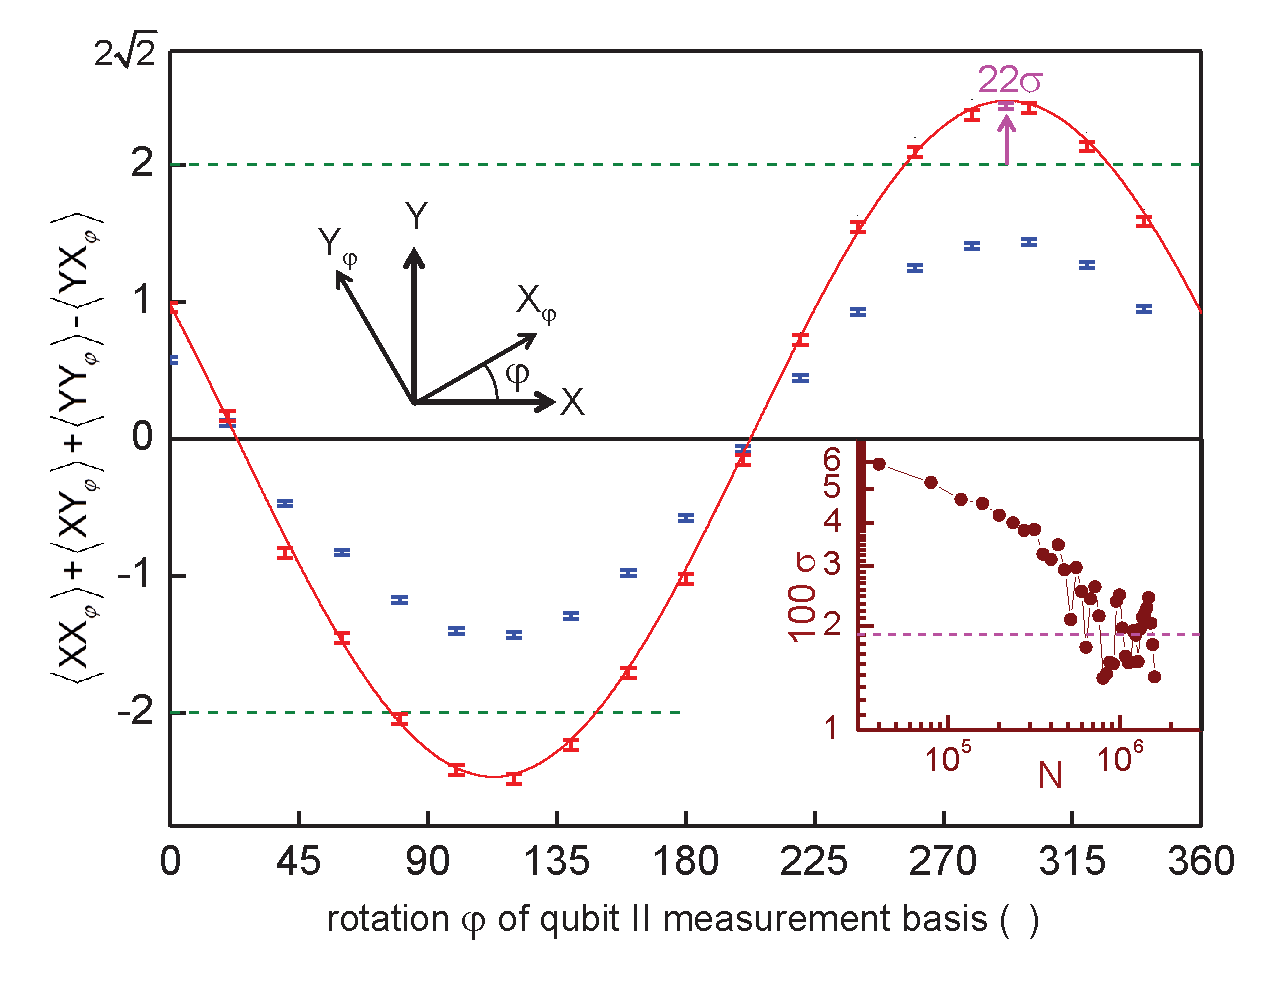
\includegraphics[width=0.8\textwidth]{./material/papers/iswap/figures/chsh}
	\end{tabular}
	\caption[]{ CHSH Bell test experiment. a) Experimental pulse sequence used (see text). b) Expectation value $\bracket{\mathrm{CHSH}}$ of the CHSH operator measured for an ensemble of identically prepared Bell states $1/\sqrt{2}(\ket{01}+e^{-i\phi}\ket{10})$, as a function of the rotation angle $\varphi$ of the qubit II measurement basis. Blue and red markers correspond to measured data uncorrected and corrected for readout errors, respectively. The solid line is the best fit of the theory. The inset shows the standard deviation $\sigma$ of the maximum value of the $\bracket{\mathrm{CHSH}}$ as a function of the sample size $N$. For large $N$, $\sigma$ is limited by a temperature induced experimental drift of the equipment (see text).}
	\label{fig:chsh}
	\label{fig:chsh_pulse_sequence}
\end{figure}


Another way to illustrate our ability to generate entangled states is to perform a so called {\it Bell test}  \citep{einstein_can_1935,bell_einstein_1964}  on our two-qubit system.

\smallskip

We follow the experimental procedure proposed by Clauser {\it et. al.} \citep{clauser_proposed_1969,freedman_experimental_1972,aspect_experimental_1982} and prepare an entangled two-qubit state of the form
%
\begin{equation}
\ket{\phi} = \frac{1}{\sqrt{2}}\left(\ket{01}+e^{-i\phi}\ket{10}\right). \label{eq:chsh_state}
\end{equation}
%
Then the expectation value of the operator
%
\begin{equation}
\mathrm{CHSH} = \mathrm{XX_{\varphi}}+\mathrm{XY_{\varphi}}+\mathrm{YY_{\varphi}}-\mathrm{YX_{\varphi}}
\end{equation}
%
is measured, where the individual operators are given as
%
\begin{eqnarray}
	\begin{array}{cccccccc}
		\mathrm{X} & = & \hat{\sigma}_x^I  &&& \mathrm{X_{\varphi}} & = & \hat{\sigma}_x^{II}\cdot \cos{\varphi}+\hat{\sigma}_y^{II} \cdot \sin{\varphi}, \\
		\mathrm{Y} & = & \hat{\sigma}_y^I&&& \mathrm{Y_{\varphi}} & = & \hat{\sigma}_y^{II}\cdot \cos{\varphi}-\hat{\sigma}_x^{II} \cdot \sin{\varphi},
	\end{array}
\end{eqnarray} 
%
with $\varphi$ the angle of rotation of the measurement basis of qubit II with respect to that of qubit I. For a non-entangled state, $|\bracket{\mathrm{CHSH}}|$  is bound by 2, whereas for an entangled state, its maximum value is $2\sqrt{2}$. 

\smallskip

The pulse sequence used for this experiment is slightly different from the previous ones: qubit II is excited in state $\ket{1}$ with a $\pi$ pulse and qubit I is brought to resonance with it for 1/4th of the swap period; then, single-qubit rotations are applied to align the qubit state with the measurement axis and $\hat{\sigma}_z^I\cdot \hat{\sigma}_z^{II}$ is measured. $\bracket{\mathrm{CHSH}}$  is finally obtained by repeating this procedure on an ensemble of up to N=1000,000 identically prepared input states $\ket{\phi}$, for the four individual operators in the CHSH equation. Figure \ref{fig:chsh} shows the protocol used as well as the results obtained. As can be seen, the expectation value $\bracket{\mathrm{CHSH}}$ varies sinusoidally as a function of the rotation angle $\varphi$. The maximum value of $\bracket{\mathrm{CHSH}}$ reaches $\approx 1.40$ and $\approx 2.52$, for uncorrected and corrected readout outcomes, respectively. Thus, uncorrected data fail to violate the non-classical boundary whereas corrected data does exceed the boundary by about 22 standard deviations. In other words, a violation of the CHSH Bell inequality is observed in our two-qubit processor although the detector efficiency loophole cannot be closed, unlike at other experiments performed with phase qubits \citep{ansmann_violation_2009}. In addition, due to the measurement time required to determine the state of each qubit and the close proximity of the two qubits, we are obviously not able to close the communication or locality loophole either. However, when accepting the general validity of quantum mechanics, the  violation of the Bell inequality in  our processor can still serve as an entanglement witness and can be regarded as a benchmark for entanglement generation.

\begin{SCfigure}[1.0][ht!]
	\centering
	\includegraphics[width=9cm]{"./data/ct5/2011_03_17 - chsh/chsh_drift"}
	\caption[]{Measured phase $\phi$ of an experimentally prepared Bell state as a function of time, over a full night. The phase exhibits an ``oscillatory'' drift of the order of $40^\circ$ being caused by temperature fluctuations.}
	\label{fig:chsh_drift}
\end{SCfigure}

\subsubsection{Errors in the Bell test} 

Besides obvious readout errors that can be corrected, the main source of errors in our Bell experiment is a temperature induced drift of the measuring equipment. Most importantly, the phase of the arbitrary waveform generator (AWG) that generates the sideband pulses for driving the qubits, drifts with respect to the phase of the microwave sources, thereby changing the phase $\phi$ of the prepared Bell state $\ket{\phi}$ and the relative angle $\varphi$ between the measurement bases of the two qubits. Figure \ref{fig:chsh_drift} demonstrates this effect by showing the evolution of the phase $\phi$ extracted from subsequent CHSH data set as those of fig. \ref{fig:chsh}, over a full night, and with the air conditioning system of the laboratory on: Oscillations of $\approx 40^\circ$, correlated with the fan activity, are observed. They correspond to a time shift of the AWG of the order of $200\;\mathrm{ps}$, which has indeed been observed independently using a fast oscilloscope. Note that data of fig. \ref{fig:chsh} had to be taken at a minimum of the temperature oscillation.

\section{Realization and Characterization of the $\sqrt{i\mathrm{SWAP}}$ Gate}

The implementation of the $\sqrt{i\mathrm{SWAP}}$ gate has already been explained in section \ref{section:Bell_states} and is recalled on fig. \ref{fig:iswap_pulse_sequence}: Qubit I is brought in resonance with qubit II during a time $t_{\sqrt{i\mathrm{SWAP}}}=1/8g$, which, for our experimental value of $2g_{qq}/2\pi = 8.3\;\mathrm{MHz}$ corresponds to $t_{\sqrt{i\mathrm{SWAP}}}\approx 30\;\mathrm{ns}$; then single-qubit Z rotations are applied to both qubits to compensate the dynamical phases $\theta_I$ and $\theta_{II}$ acquired during the swapping, as given by the first part of the operator (\ref{eq:swap_evolution_operator_main}). Again, the angles of these Z rotations are pre-calibrated by applying the gate to the input state $(\ket{00}+\ket{01})/\sqrt{2}$, comparing the phases of the output state to the desired ones and changing the Z pulse amplitudes accordingly. The goal is now to quantify the fidelity of our gate and to analyze the error sources limiting this fidelity.	This analysis  is more demanding than simply demonstrating a violation of a Bell inequality, or than measuring by quantum state tomography particular entangled states with a high fidelity. The goal is now to demonstrate that the targeted evolution operator is implemented with a high fidelity whatever the chosen input state for the register. In this section, we explain the so-called quantum process tomography method used to reach that goal. In order to characterize the gate itself and not the protocol used to characterize it, we are led to model the drive errors and to measure them in a pre-calibration experiment. This allows us to remove the preparation and tomography errors from the gate characterization and to obtain an intrinsic $\sqrt{i\mathrm{SWAP}}$ gate fidelity (contrary to the state fidelities reported above that contained also tomographic errors).

\begin{figure}[hb!]
	\centering
		\includegraphics[width=0.8\textwidth]{./material/figures/measurement/qubit_iswap_full}
	\caption{Experimental pulse sequence used for implementing the two-qubit $\sqrt{i\mathrm{SWAP}}$ gate. The sequence shown for an exemplary input state $\ket{10}$ consists in exciting the first qubit to the state $\ket{1}$, bringing the qubits in resonance for a time $t=1/8g$, separating them and compensating the acquired dynamical phases by using two single-qubit $Z$-pulses. Finally, optional tomographic pulses are applied before reading out the qubit state at the optimal readout frequencies of the qubits.}
	\label{fig:iswap_pulse_sequence}
\end{figure}

\subsection{Principle of Quantum Process Tomography}

{\it Quantum process tomography} \citep{poyatos_complete_1997} is an ensemble of methods allowing  one to fully characterize any experimental quantum process. The particular approach that we use and present below is called {\it standard quantum process tomography} (SQPT), but there exist other methods such as ancilla-assisted quantum process tomography \citep{dur_nonlocal_2001,dariano_quantum_2001,altepeter_ancilla-assisted_2003} that we will not discuss.

\subsubsection{Theoretical Description of a Quantum Process}

As explained in section \ref{section:master_equation}, any quantum process on an n-qubit system can be described by a set of at most $N=4^n$ Kraus operators, as given by eq. (\ref{eq:kraus_representation}):
%
\begin{equation}
\begin{mathcal}E\end{mathcal}(\rho) = \sum\limits_i^{N} E_i \rho E_i^\dagger \label{eq:kraus_representation_2}.
\end{equation}
%
Now, if we express these operators $E_i$ in a fixed operator basis $\tilde{E}_j$ such that $E_i = \sum_j^N a_{ij} \tilde{E}_{j}$, we can rewrite eq. (\ref{eq:kraus_representation_2}) as

\begin{eqnarray}
 \mathcal{E}(\rho) & = & \sum\limits_i^N \sum\limits_j^{N} a_{ij} \tilde{E}_j \;\rho\; \sum\limits_k^{N} a_{ik}^* \tilde{E}_k^\dagger \\
& = & \sum\limits_{j,k}^{N}\tilde{E}_j \; \rho \; \tilde{E}_k^\dagger \sum\limits_i^N a_{ij} a_{ik}^* \\
& = & \sum\limits_{j,k}^{N}\tilde{E}_j \; \rho \; \tilde{E}_k^\dagger \; \chi_{jk}, \label{eq:process_chi_representation}
\end{eqnarray}
where we defined $\chi_{jk} = \sum\limits_i a_{ij} a_{ik}^*$. Equation (\ref{eq:process_chi_representation}) is the $\chi$-matrix representation of the quantum process in the basis $\{\tilde{E}_j\}$, which contains all the information about the process.

\subsubsection{Implementation of Standard Quantum Process Tomography}

The goal of SQPT is to obtain the $N^2$ independent real coefficients of the $\chi$-matrix -- or any other complete parametrization of the process -- from a set of $N$ experimentally measured output matrices $\{\mathcal{E}(\rho_i)\}$, given a set of $N$ known and independent  input matrices $\{\rho_i\}$. Note that measuring also the  $N$ input matrices might be required to know them with a sufficient accuracy, in particular when errors occur in their preparation. More precisely, one implements SQPT for a n-qubit system by using the following procedure:

\begin{enumerate}
\item Choose a set of $N$ operators $\tilde{E}_j$ that forms a full basis for the operators acting on the n-qubit Hilbert space. One usually chooses $\tilde{E}_{j_1,j_2 \hdots j_n} = \hat{\sigma}_{j_1}\otimes \hat{\sigma}_{j_2}\hdots\otimes\hat{\sigma}_{j_n}$, where $\hat{\sigma}_j$ are the single-qubit Pauli operators, i.e. $j\in\{I,X,Y,Z\}$.
\item Choose $N$ pure quantum states $\ket{\phi_i}$ such that the basis $\{\ket{\phi_1}\bra{\phi_1}$, $\ket{\phi_1}\bra{\phi_2}\hdots$, $\ket{\phi_{N}}\bra{\phi_{N-1}},\ket{\phi_{N}}\bra{\phi_{N}}\}$ spans the whole Hilbert space of input density matrices $\rho$. One usually chooses $\ket{\phi} \in \{\ket{0},\ket{1},(\ket{0}+\ket{1})/\sqrt{2},(\ket{0}+i\ket{1})/\sqrt{2}\}^{\otimes n}$, where $^{\otimes n}$ denotes the n-dimensional Kronecker product of all possible permutations.
\item Prepare each of the chosen input states $\rho_i = \ket{\phi_i}\bra{\phi_i}$, apply the gate operation, and determine the output states $\mathcal{E}(\ket{\phi_i}\bra{\phi_i})$ by quantum state tomography. Optionally, perform quantum state tomography of the prepared state $\rho_i$ as well to determine experimental preparation and tomography errors.
\item After having determined the $\rho_i$ and $\mathcal{E}(\rho_i)$, write $\mathcal{E}(\rho_i) = \sum_j \lambda_{ij} \tilde{\rho}_j$  in a complete basis $\{\tilde{\rho}_1,\hdots,\tilde{\rho}_{2^n}\}$ for the $2^n$x$2^n$ matrices. Usually one chooses $\tilde{\rho}_j$ matrices with only one element equal to one and all the others equal to zero.
 Calculate the $N^{\otimes 4}$ tensor $\beta_{jk}^{mn}$ defined by $\tilde{E}_m \tilde{\rho}_j \tilde{E}_n^\dagger = \sum_k \beta_{jk}^{mn}\tilde{\rho}_k$, and insert this definition into eq. (\ref{eq:process_chi_representation}) to obtain
%
\begin{eqnarray}
\sum\limits_k \lambda_{ik} \tilde{\rho}_k & = & \sum\limits_{m,n} \chi_{mn} \sum\limits_k \beta_{ik}^{mn} \tilde{\rho}_k .
\end{eqnarray}
%
Equating the two sides yields $\lambda_{ik} = \sum_{m,n}\beta_{ik}^{mn}\; \chi_{mn}$, which, by linear inversion,  gives $\chi$.

\end{enumerate}



\smallskip

Similar to quantum state tomography, experimental errors occurring during quantum process tomography can produce a process matrix $\chi$ that is {\it non-physical} in the sense that the resulting quantum process does not obey the three axioms stated in section \ref{section:master_equation}. Therefore, we render the obtained $\chi$ matrix physical by numerically searching the  physical process matrix $\chi_{ph}$ that has the smallest distance $d=\|\chi-\chi_{ph}\|$  to the original one, using e.g. the Hilbert-Schmidt distance $\|A-B\| = \mathrm{Tr}(|A-B|)^2$. 

\subsubsection{Kraus Representation of the Process}

To go back from the $\chi$-matrix representation of the quantum process to the Kraus form given by eq. (\ref{eq:kraus_representation}), one writes each process-independent operator $\tilde{E}_i$ as a sum of all the Kraus operators $E_l$, such that
%
\begin{equation}
	\tilde{E}_i = \sum\limits_l a_{il}\; E_l. \label{eq:kraus_operators_decomposition}
\end{equation}
%
Inserting eq. (\ref{eq:kraus_operators_decomposition}) into eq. (\ref{eq:process_chi_representation}), we obtain
%
\begin{eqnarray}
\begin{mathcal}E\end{mathcal}(\rho) & = & \sum\limits_{j,k}\chi_{jk}\sum\limits_{l,m} a_{jl}a_{km}^* E_l \rho E_m^\dagger   \label{eq:process_chi_transformed} \\
& = & \sum\limits_i E_i \rho E^\dagger_i.
\end{eqnarray}
%
One finds hence the condition $\sum\limits_{j,k} \chi_{jk}a_{jl}a_{km}^* = \delta_l^m$, or, written in matrix form $A\chi A^\dagger = \mathrm{I}$, which is fulfilled if $A$ is the matrix of eigenvectors of $\chi$, multiplied by the square root of the corresponding diagonal matrix of eigenvalues. It is thus easy to obtain the Kraus representation of the quantum process by diagonalizing the Hermitian matrix $\chi$.

\smallskip

The Kraus operator form of the quantum process can be useful since it shows in a simple way the different operators acting on the density matrix $\rho$. By ordering them as a function of their corresponding eigenvalues, one obtains the different unitary and non-unitary processes acting together on the density matrix $\rho$, ordered by importance.

\subsection{Modeling and Determination of Tomography Errors}

As already briefly mentioned, quantum process tomography (resp. quantum state tomography) used for characterizing a two-qubit gate (resp. state) requires additional manipulation steps that adds errors which should not be taken as gate errors (resp. state errors). In our experiment, the systematic single-qubit  pulse errors impact both the prepared input states for process tomography, and the tomographic pulses themselves. In the first case, it is not a problem because the input states can also be measured and their discrepancy with respect to the targeted input states does not impact the process description. On the contrary, tomographic errors are a problem and should be removed from the gate description.
Consequently, we pre-determine our pulse errors in the following way: We choose a model for the errors, which we discuss in the following two sections, and fit it to a large set of measured data, as presented afterwards.


\subsubsection{Leakage Out of the Computational Hilbert-Space}

\begin{figure}[ht!]
	\centering
	\includegraphics[width=\textwidth]{./material/figures/2-qubit-processor/swap_energy_levels}
	\caption{Energy level diagram illustrating the possible swapping interactions of two three-level Transmon qubits. Resonant transitions are a)  the $\ket{01}\leftrightarrow\ket{10}$ and $\ket{12}\leftrightarrow\ket{21}$ transitions at $\omega_{01}^I = \omega_{01}^{II}$ (with swapping frequencies $g_{qq}$ and $2g_{qq}$, respectively), b) the $\ket{11}\leftrightarrow\ket{20}$ transition at $\omega_{12}^{I} = \omega_{01}^{II}$ and c) the $\ket{11}\leftrightarrow\ket{02}$ transition at $\omega_{01}^I = \omega_{12}^{II}$ (both with a swapping frequency $\sqrt{2}g_{qq}$).}
	\label{fig:swap_energy_levels}
\end{figure}

\smallskip

\begin{figure}[ht!]
	\centering
	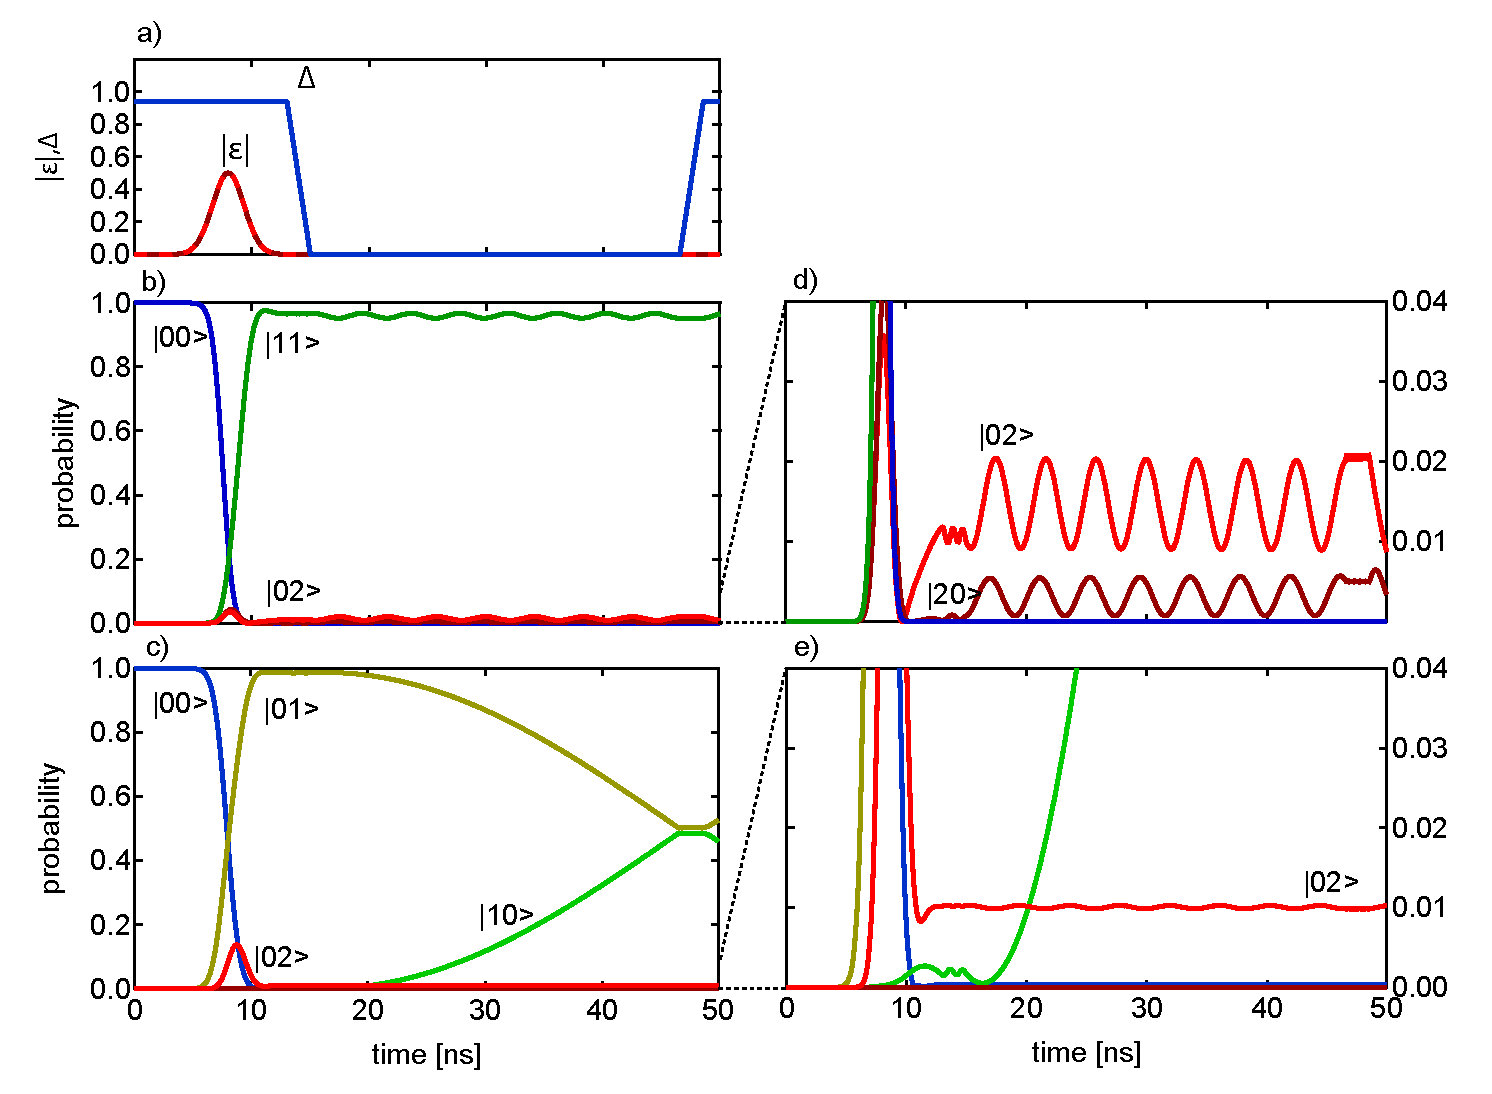
\includegraphics[width=\textwidth]{./data/simulation/three_level_swap/plots}
	\caption{a1) Drive and flux waveforms for a simulated $\sqrt{i\mathrm{SWAP}}$ gate between two three-level Transmons. a2/a3) State occupation probabilities during the simulation for the input states $\ket{01}$ (a2) and $\ket{11}$ (a3). b1/b2) show a zoom-in on the two figures a2/a3). In both cases, a small excitation of the higher Transmon level $\ket{2}$ can be observed in the simulation. For the $\ket{11}$ input state, an oscillation between the states $\ket{11}$ and $\ket{02}$/$\ket{20}$ can be observed, which is an unwanted effect. }
	\label{fig:swap_3_level_data}
\end{figure}

An error source that we estimate here is the leakage to the higher Transmon level $\ket{2}$, as discussed in section \ref{section:charge_driving}. This error can occur while driving the qubits or due to the swapping interaction between the $\ket{11}\leftrightarrow\ket{20}$ and $\ket{11}\leftrightarrow\ket{02}$ states of the three-level two-qubit Hamiltonian given by eq. (\ref{eq:three_level_interaction_hamiltonian}), as illustrated in fig. \ref{fig:swap_energy_levels}. To quantify this leakage, we perform a simulation of our $\sqrt{i\mathrm{SWAP}}$ gate between two three-level Transmons, using the measured qubit parameters. We don't include decoherence that tends to lower the leakage and instead use the same Hamiltonian as in section \ref{section:three_level_simulation}. Just as in our experiment, we generate the 16 different input states listed above using simulated Gaussian drive pulses with a rise time of $\delta t = 4\;\mathrm{ns}$ while the qubits are detuned by $\Delta_{qq}/2\pi = 150\;\mathrm{MHz}$. We then reduce the detuning to $\Delta_{qq} = 0$ during $t_\mathrm{SWAP}\approx 31 \;\mathrm{ns}$ using a simulated flux pulse with a $2\;\mathrm{ns}$ rise time, as shown in fig. \ref{fig:swap_3_level_data}. We compute numerically the fidelity of the output state with an output state obtained from the ideal $\sqrt{i\mathrm{SWAP}}$ operation applied to the simulated input state. By examining the output density matrices we can then give an upper bound for the leakage error into the state $\ket{2}$, which in our case is $\approx 1.5\;\%$. Figure \ref{fig:swap_3_level_data} exemplarily shows the simulated state occupation probabilities for the two input states $\ket{01}$ and $\ket{11}$. In both cases, a small excitation of the $\ket{02}$ and $\ket{20}$ Transmon states can be observed at the end of the sequence. The $\ket{11}$ input state, which should not be affected by the SWAP operation, shows a small oscillation due to the coupling to the $\ket{02}$ state.

\smallskip

Since the obtained overall error is small, we neglect the leakage to state $\ket{2}$ in the error model that we present now. Please note that the results of this simulation should be regarded as a rough estimate since the inclusion of higher Transmon levels would certainly alter the obtained error boundaries.

\subsubsection{Modeling and Determining Pulse Errors} \label{section:tomographic_errors}

The error model we use includes errors both in the preparation of the states (index $\mathrm{prep}$) and in
the tomographic pulses (index $\mathrm{tomo}$). The errors included are angular
errors $\varepsilon_{\mathrm{I,II}}^{\mathrm{prep}}$ on the nominal
$\pi$ rotations around $X_{\mathrm{I,II}}$, $\eta_{\mathrm{I,II}}^{\mathrm{prep,tomo}}$and
$\delta_{\mathrm{I,II}}^{\mathrm{prep,tomo}}$ on the nominal $\pi/2$
rotations around $X_{\mathrm{I,II}}$ and $Y_{\mathrm{I,II}}$, a
possible departure $\xi_{\mathrm{I,II}}$ from orthogonality of $\left(\overrightarrow{X_{\mathrm{I}}},\overrightarrow{Y_{\mathrm{I}}}\right)$ and $\left(\overrightarrow{X_{\mathrm{II}}},\overrightarrow{Y_{\mathrm{II}}}\right)$,
and a possible rotation $\mu_{\mathrm{I,II}}$ of the tomographic
$XY$ frame with respect to the preparation one. The rotation operators
used for preparing the states and doing their tomography are thus
given by

\[
\begin{array}{c}
X_{\mathrm{I,II}}^{\mathrm{prep}}(\pi)=e^{-\mathrm{i}\left(\pi+\varepsilon_{\mathrm{I,II}}^{\mathrm{prep}}\right)\hat{\sigma}_{\mathrm{x}}^{\mathrm{I,II}}/2},\\
X_{\mathrm{I,II}}^{\mathrm{prep}}(-\pi/2)=e^{+\mathrm{i}\left(\pi/2+\eta_{\mathrm{I,II}}^{\mathrm{prep}}\right)\hat{\sigma}_{\mathrm{x}}^{\mathrm{I,II}}/2},\\
Y_{\mathrm{I,II}}^{\mathrm{prep}}(\pi/2)=e^{-\mathrm{i}\left(\pi/2+\delta_{\mathrm{I,II}}^{\mathrm{prep}}\right)\left[\mathrm{cos}\left(\xi_{\mathrm{I,II}}\right)\hat{\sigma}_{\mathrm{y}}^{\mathrm{I,II}}\mathrm{-sin}\left(\xi_{\mathrm{I,II}}\right)\hat{\sigma}_{\mathrm{x}}^{\mathrm{I,II}}\right]/2},\\
X_{\mathrm{I,II}}^{\mathrm{tomo}}(\pi/2)=e^{-\mathrm{i}\left(\pi/2+\eta_{\mathrm{I,II}}^{\mathrm{tomo}}\right)\left[\mathrm{\mathrm{sin}\left(\mu_{I,II}\right)\hat{\sigma}_{x}^{I,II}+cos}\left(\mu_{\mathrm{I,II}}\right)\hat{\sigma}_{\mathrm{y}}^{\mathrm{I,II}}\right]/2},\\
Y_{\mathrm{I,II}}^{\mathrm{tomo}}(-\pi/2)=e^{+\mathrm{i}\left(\pi/2+\delta_{\mathrm{I,II}}^{\mathrm{tomo}}\right)\left[\mathrm{cos}\left(\mu_{\mathrm{I,II}}+\xi_{\mathrm{I,II}}\right)\hat{\sigma}_{\mathrm{y}}^{\mathrm{I,II}}\mathrm{-sin}\left(\mu_{\mathrm{I,II}}+\xi_{\mathrm{I,II}}\right)\hat{\sigma}_{x}^{\mathrm{I,II}}\right]/2}.\end{array}\]

We determine these error parameters by fitting the model to a large set of measured data. A natural choice is to use the sixteen input states that we use for the quantum process tomography. These input states are given as $\{ \rho_{\mathrm{in}}^{\mathrm{e}}=U\left|0\right\rangle \left\langle 0\right|U^{\dagger}\} $
with 
%
\begin{equation}
\{ U\} =\{I_{\mathrm{I}}, X_{\mathrm{I}}^{\mathrm{prep}}(\pi), Y_{\mathrm{I}}^{\mathrm{prep}}(\pi/2),X_{\mathrm{I}}^{\mathrm{prep}}(-\pi/2)\}\otimes\{I_{\mathrm{II}},X_{\mathrm{II}}^{\mathrm{prep}}(\pi),Y_{\mathrm{II}}^{\mathrm{prep}}(\pi/2),X_{\mathrm{II}}^{\mathrm{prep}}(-\pi/2)\},
\end{equation}
%
and each input state yields a Pauli set $\left\{ \left\langle P_{\mathrm{k}}^{\mathrm{e}}\right\rangle =Tr\left(\rho_{\mathrm{in}}^{\mathrm{e}}P_{\mathrm{k}}^{\mathrm{e}}\right)\right\} $
with $\left\{ P_{\mathrm{k}}^{\mathrm{e}}\right\} =\{I_{\mathrm{I}},X_{\mathrm{I}}^{\mathrm{e}},Y_{\mathrm{I}}^{\mathrm{e}},Z_{\mathrm{I}}\}\otimes\{I_{\mathrm{II}},X_{\mathrm{II}}^{\mathrm{e}},Y_{\mathrm{II}}^{\mathrm{e}},Z_{\mathrm{II}}\}$,
$X^{\mathrm{e}}=Y^{\mathrm{tomo}}(-\pi/2)^{\dagger}\hat{\sigma}_{z}Y^{\mathrm{tomo}}(-\pi/2)$,
and $Y^{\mathrm{e}}=X^{\mathrm{tomo}}(\pi/2)^{\dagger}\hat{\sigma}_{\mathrm{z}}X^{\mathrm{tomo}}(\pi/2)$.

\begin{figure}[htp!]
	\centering
	\includegraphics[width=0.9\textwidth]{./material/papers/iswap/submission1/error_model}
	\caption{Fitting of the pulse errors at state preparation and tomography. Measured
(red) and fitted (blue - see text) Pauli sets $\left\langle P_{\mathrm{k}}^{\mathrm{e}}\right\rangle $
for the sixteen targeted input states $\{\left|0\right\rangle ,\left|1\right\rangle ,\left|0\right\rangle +\left|1\right\rangle ,\left|0\right\rangle +i\left|1\right\rangle \}^{\otimes2}$.
The $\{II,IX,IY,IZ,XI,...\}$ operators indicated on the abscissa are
the targeted operators and not those actually measured (due to tomographic
errors).}
	\label{fig:fit_Pulse_Errors}
\end{figure}

\smallskip

Figure \ref{fig:fit_Pulse_Errors} shows the 16 measured Pauli sets as well as the best fit to the data, which yields $\varepsilon_{\mathrm{I}}^{\mathrm{prep}}=-1\text{\textdegree}$,
$\varepsilon_{\mathrm{II}}^{\mathrm{prep}}=-3\text{\textdegree}$,
$\eta_{\mathrm{I}}^{\mathrm{prep}}=3\text{\textdegree}$, $\mathrm{\eta}_{\mathrm{II}}^{\mathrm{prep}}=4\text{\textdegree}$,
$\delta_{\mathrm{I}}^{\mathrm{prep}}=-6\text{\textdegree}$, $\delta_{\mathrm{II}}^{\mathrm{prep}}=-3\text{\textdegree}$,
$\eta_{\mathrm{I}}^{\mathrm{tomo}}=-6\text{\textdegree}$, $\eta_{\mathrm{II}}^{\mathrm{tomo}}=-4\text{\textdegree}$,
$\lambda_{\mathrm{I}}^{t\mathrm{omo}}=12\text{\textdegree}$, $\lambda_{\mathrm{II}}^{\mathrm{tomo}}=5\text{\textdegree}$,
$\xi_{\mathrm{I}}=1\text{\textdegree}$, $\xi_{\mathrm{II}}=-2\text{\textdegree}$,
and $\mu_{\mathrm{I}}=\mu_{\mathrm{II}}=-11\text{\textdegree}$. 

\begin{figure}[p]
	\centering
		\includegraphics[width=1.0\textwidth]{"./data/ct5/2011_04_21 - grover and tomo/good_data/process -matrices 1"}
	\caption{Experimental input and output density matrices used for quantum process tomography of our $\sqrt{i\mathrm{SWAP}}$ gate. Shown are the input/output pairs for the 16 different input states indicated below each matrix and the corresponding output matrices with their state fidelities. The corresponding ideal matrices are overlaid in black. (part I/II)}
	\label{fig:process_matrices_1}
\end{figure}

\begin{figure}[p]
	\centering
		\includegraphics[width=1\textwidth]{"./data/ct5/2011_04_21 - grover and tomo/good_data/process -matrices 2"}
	\caption{}
	\label{fig:process_matrices_2}
\end{figure}

\subsection{Experimental Chi matrix and Gate Fidelity}

\begin{figure}[ht!]
	\centering
		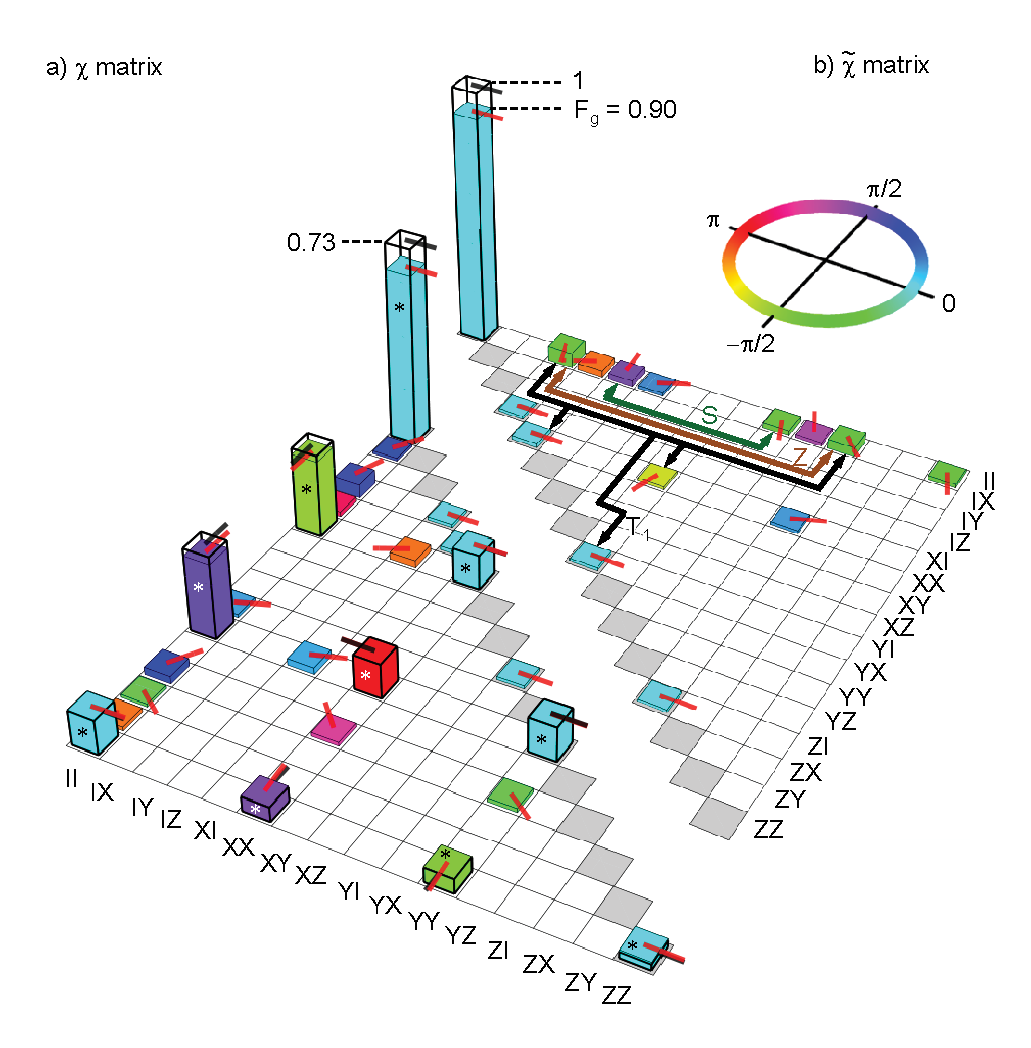
\includegraphics[width=1.\textwidth]{./material/papers/iswap/figures/chi_matrix_and_error_process}
	\caption{Reconstructed $\chi$ process matrix of our implementation of the $\sqrt{i\mathrm{SWAP}}$ quantum gate. a) Superposition of the ideal (empty thick bars) and experimental
(color filled bars) lower part of the Hermitian matrix $\chi$ (elements
below 1\% not shown). Each complex matrix element is represented by
a bar with height proportional to its modulus and a red phase pointer
at the top of the bar (as well as a filling color for experiment)
giving its argument (top left inset). Expected peaks are marked by
a star. b) Error process matrix $\tilde{\chi}=\chi\cdot\chi_{id}^{-1}$. The colored arrows grouping different elements of $\tilde{\chi}$ indicate unitary and non-unitary error processes to which the corresponding matrix elements can be associated.}
	\label{fig:chi_matrix_and_errors}
\end{figure}

We can now perform the standard process tomography of our two-qubit gate by following the procedure outlined in the previous sections: the 16 input and 16 output Pauli sets are measured by standard quantum state tomography. 
Knowing the tomographic errors and thus $\left\{ \left\langle P_{\mathrm{k}}^{\mathrm{e}}\right\rangle \right\} $,
we then invert the linear relation $\left\{ \left\langle P_{\mathrm{k}}^{\mathrm{e}}\right\rangle =Tr\left(\rho P_{\mathrm{k}}^{\mathrm{e}}\right)\right\} $
to find the $16\times16$ matrix $B$ that links the vector $\overrightarrow{\left\langle P_{\mathrm{k}}^{\mathrm{e}}\right\rangle }$
to the columnized density matrix $\overrightarrow{\rho}$, i.e. $\overrightarrow{\rho}=B.\overrightarrow{\left\langle P_{\mathrm{k}}^{\mathrm{e}}\right\rangle }$.
The matrix $B$ is finally applied to the measured 16 input and
16 output Pauli sets to find the 16 $(\rho_{\mathrm{in},},\rho_{\mathrm{out}})_{\mathrm{k}}$
couples to be used for calculating the gate map. Figures \ref{fig:process_matrices_1} and \ref{fig:process_matrices_2} show the experimentally determined $(\rho_{\mathrm{in},},\rho_{\mathrm{out}})_{\mathrm{k}}$ pairs, with a comparison to the ideal ones. The targeted input states are annotated below the corresponding $\rho_{in}$. The trace fidelity (\ref{eq:quantum_trace_fidelity}) between the experimental and ideal matrices is indicated above.

\smallskip

From these input/output matrices, we calculate the $\chi$ matrix of the quantum process by the method described above. This $\chi$ matrix is shown in fig. \ref{fig:chi_matrix_and_errors}, together with matrix $\chi_{id}$ of an ideal  $\sqrt{i\mathrm{SWAP}}$ process. The fidelity of the gate process is $F_g=\mathrm{Tr}(\chi \chi_{id})=0.90$.

\smallskip

\begin{figure}[ht!]
	\centering
		\includegraphics[width=1.\textwidth]{"./data/ct5/2011_04_21 - grover and tomo/good_data/process_kraus_operators"}
	\caption{Experimental Kraus operators of the implemented $\sqrt{i\mathrm{SWAP}}$ gate, as obtained from the diagonalization of the $\chi_{exp}$ matrix in fig. \ref{fig:chi_matrix_and_errors}. Shown are only the four operators with the largest eigenvalues, which together account for $>99.9 \%$ of the operator weights and therefore describe the process with very good accuracy.}
	\label{fig:kraus_operators}
\end{figure}

From the experimental $\chi$ matrix, we then calculate the Kraus operators. In our case, the 4 largest eigenvalues $\lambda_i$ of $\chi$ (for which $\sum\limits_i \lambda_i = 1$) sum up to a value $>0.999$ and therefore suffice to describe the process with high accuracy. The corresponding 4 Kraus operators with their eigenvalues are shown in fig. \ref{fig:kraus_operators}. As can be seen, the operator associated to the largest eigenvalue $\lambda=0.909$ corresponds closely to the unitary $\sqrt{i\mathrm{SWAP}}$ operator. The other operators are largely non-unitary and describe the decoherence in the quantum process. Since the Kraus operators contain the same information on the quantum process as the $\chi$-matrix, we can fit the observed operators to a decoherence model of the quantum process to obtain an estimate of the relaxation and dephasing rates. However, since we already performed the same operation above using the $\chi$-matrix, we will not repeat it here.

\subsection{Gate Error Analysis}

 To better visualize the discrepancy between the experimental and ideal $\chi$ matrices, the error process matrix $\tilde{\chi} = \chi\cdot\chi_{id}^{-1}$ is also shown in fig. \ref{fig:chi_matrix_and_errors}. This matrix that would simply be the identity matrix if the gate was perfect, displays the errors in a rather cryptic way. To understand the origin of the errors, we finally fit to $\tilde{\chi}$ a master equation model of the quantum process, which involves a frequency offset when performing the swapping interaction, errors in the amplitude of the compensating $Z$ pulses applied after the swap, as well as individual relaxation and dephasing super-operators. The relaxation and dephasing rates employed in the simulation are the same as those discussed in section \ref{section:creation_of_entanglement}, whereas the unitary error parameters are fitted to maximize the fidelity between the simulated and measured $\tilde{\chi}$ matrices. Using this technique, we infer an error budget of the quantum process that quantifies the contributions of individual error sources.

We find a total gate error of $10 \%$, where we can attribute $8\%$ of the errors to relaxation and decoherence during the process and $2\%$ to unitary gate errors. By plotting the different $\tilde{\chi}$ matrices that would correspond to each error source if it was alone, we see which matrix element is produced in the matrix. This allows us to localize the different error sources in the measured $\tilde{\chi}$, as shown by the arrows in fig. \ref{fig:chi_matrix_and_errors}.

\section{Conclusion}

In this chapter we demonstrated that we can implement a universal set of quantum gates on our two-qubit processor. We created and characterized entangled two-qubit states, performed quantum state tomography, implemented the $\sqrt{i\mathrm{SWAP}}$ quantum gate with a fidelity of $90\%$ and analyzed the most important error sources of the gate operation.

\smallskip

In the next chapter, we use the set of universal gates to run a simple quantum search algorithm on our two-qubit processor, showing that we are able to demonstrate quantum speed-up for a real-world problem, albeit at a scale which is not yet practically useful.
